\documentclass[tikz, border=1mm]{standalone}
\usepackage{tikz} 
\usetikzlibrary{arrows.meta}
\usepackage{pgfplots}

\begin{document}

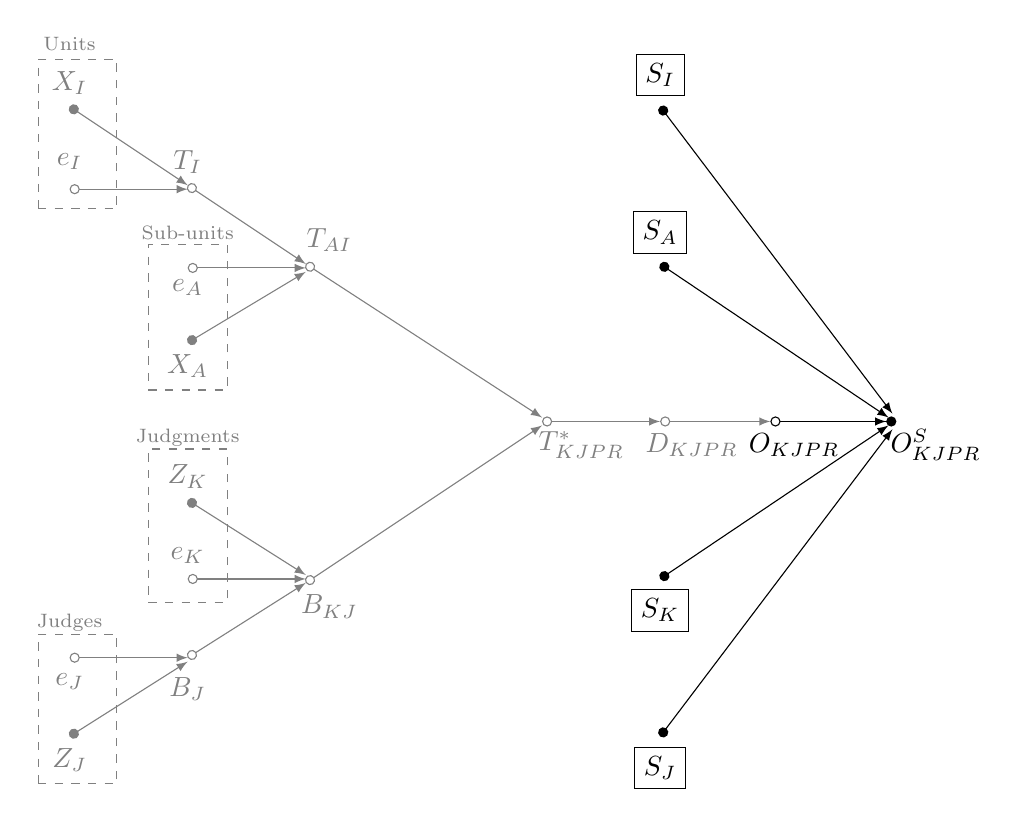
\begin{tikzpicture}

    % complete outcome
    \node at (3.20,0.7) {$O_{{KJPR}}$}; %[gray]
    
    % discriminal difference
    \node[gray] at (1.9,0.7) {$D_{{KJPR}}$}; %[gray]
    %\draw[{Circle[open]}-{latex}{Circle},gray](1.5,1) to (3,1); %,gray
    \draw[{Circle[open]}-{latex},gray](1.5,1) to (2.9,1); %,gray
    
    % "perceived" discriminal process for vector of stimulus
    \node[gray] at (0.5,0.7) {$T^{*}_{KJPR}$}; %[gray]
    \draw[{Circle[open]}-{latex},gray](0,1) to (1.5,1); %,gray

    % "true" discriminal process for sub-unit
    \node[gray] at (-2.7,3.3) {$T_{AI}$}; %[gray]
    \draw[{Circle[open]}-{latex},gray](-3,3) to (0,1.05); %,gray

    % "true" judgments' bias k_{j}
    \node[gray] at (-2.7,-1.35) {$B_{KJ}$}; %[gray]
    \draw[{Circle[open]}-{latex},gray](-3,-1.05) to (0,0.95); %,gray

    %%%%%%%%%%%%%%%%%%%%%%%%%%%%%%%%%%%%%%%%%%%%%%%%%%%%%%

    % "true" discriminal process of unit
    \node[gray] at (-4.5,4.3) {$T_{I}$}; %[gray]
    \draw[{Circle[open]}-{latex},gray](-4.5,4) to (-3,3); %,gray

    % sub-units error
    \node[gray] at (-4.5,2.7) {$e_{A}$}; %[gray]
    \draw[{Circle[open]}-{latex},gray](-4.5,2.95) to (-3,2.95); %,gray
    
    % predictors for sub-unit
    \node[gray] at (-4.5,1.7) {$X_{A}$}; %[gray]
    \draw[{Circle}-{latex},gray](-4.5,2) to (-3,2.90); %,gray

    % sub-units' clsuter
    \node[font=\scriptsize,gray] at (-4.5,3.4) {Sub-units}; %,gray
    \draw[dashed,gray] (-5,1.4)--(-4,1.4)--(-4,3.25)--(-5,3.25)--(-5,1.4); %,gray

    %%%%%%%%%%%%%%%%%%%%%%%%%%%%%%%%%%%%%%%%%%%%%%%%%%%%%%

    % predictors for units
    \node[gray] at (-6,5.3) {$X_{I}$}; %[gray]
    \draw[{Circle}-{latex},gray](-6,5) to (-4.5,4); %,gray

    % units trait error
    \node[gray] at (-6,4.3) {$e_{I}$}; %[gray]
    \draw[{Circle[open]}-{latex},gray](-6,3.95) to (-4.5,3.95); %,gray

    % units' cluster
    \node[font=\scriptsize,gray] at (-6,5.8) {Units}; %,gray
    \draw[dashed,gray] (-6.4,3.7)--(-5.4,3.7)--(-5.4,5.6)--(-6.4,5.6)--(-6.4,3.7); %,gray

    %%%%%%%%%%%%%%%%%%%%%%%%%%%%%%%%%%%%%%%%%%%%%%%%%%%%%%

    % predictors for judgments 
    \node[gray] at (-4.5,0.3) {$Z_{K}$}; %[gray]
    \draw[{Circle}-{latex},gray](-4.5,0) to (-3,-0.95); %,gray
    
    % judgments' bias error
    \node[gray] at (-4.5,-0.7) {$e_{K}$}; %[gray]
    \draw[{Circle[open]}-{latex},gray](-4.5,-1) to (-3,-1); %,gray

    % judges' bias
    \node[gray] at (-4.5,-2.4) {$B_{J}$}; %[gray]
    \draw[{Circle[open]}-{latex},gray](-4.5,-2) to (-3,-1.05); %,gray

    % judgments' cluster
    \node[font=\scriptsize,gray] at (-4.5,0.8) {Judgments}; %,gray
    \draw[dashed,gray] (-5,-1.3)--(-4,-1.3)--(-4,0.65)--(-5,0.65)--(-5,-1.3); %,gray

    %%%%%%%%%%%%%%%%%%%%%%%%%%%%%%%%%%%%%%%%%%%%%%%%%%%%%%

    % predictors for judges' bias
    \node[gray] at (-6,-3.3) {$Z_{J}$}; %[gray]
    \draw[{Circle}-{latex},gray](-6,-3) to (-4.5,-2.05); %,gray

    % judges' bias error
    \node[gray] at (-6,-2.3) {$e_{J}$}; %[gray]
    \draw[{Circle[open]}-{latex},gray](-6,-2) to (-4.5,-2); %,gray

    % judges' cluster
    \node[font=\scriptsize,gray] at (-6,-1.55) {Judges}; %,gray
    \draw[dashed,gray] (-6.4,-3.6)--(-5.4,-3.6)--(-5.4,-1.7)--(-6.4,-1.7)--(-6.4,-3.6); %,gray

    %%%%%%%%%%%%%%%%%%%%%%%%%%%%%%%%%%%%%%%%%%%%%%%%%%%%%%
    
    % units sampling mechanism
    \node[rectangle,draw] at (1.5,5.4) {$S_{I}$}; %,gray
    \draw[{Circle}-{latex}](1.5,5) to (4.45,1.1); %,gray
    
    % units sample size
    %\node at (0,5.3) {$n_{I}$}; %[gray]
    %\draw[{Circle}-{latex}](0,4.95) to (1.5,4.95); %,gray

    % subunits sampling mechanism
    \node[rectangle,draw] at (1.5,3.4) {$S_{A}$}; %,gray
    \draw[{Circle}-{latex}](1.5,3) to (4.4,1.05); %,gray
    
    % subunits sample size
    %\node at (0,3.3) {$n_{A}$}; %[gray]
    %\draw[{Circle}-{latex}](0,2.95) to (1.5,2.95); %,gray

    % judgments sampling mechanism
    \node[rectangle,draw] at (1.5,-1.4) {$S_{K}$}; %,gray
    \draw[{Circle}-{latex}](1.5,-1) to (4.4,0.95); %,gray
    
    % judgments sample size
    %\node at (0,-1.3) {$n_{K}$}; %[gray]
    %\draw[{Circle}-{latex}](0,-0.95) to (1.5,-0.95); %,gray

    % judges sampling mechanism
    \node[rectangle,draw] at (1.5,-3.4) {$S_{J}$}; %,gray
    \draw[{Circle}-{latex}](1.5,-3) to (4.45,0.90); %,gray
    
    % judges sample size
    %\node at (0,-3.3) {$n_{J}$}; %[gray]
    %\draw[{Circle}-{latex}](0,-2.95) to (1.5,-2.95); %,gray

    % sample outcome
    \node at (5,0.7) {$O^{S}_{{KJPR}}$}; %[gray]
    \draw[{Circle[open]}-{latex}{Circle}](2.9,1) to (4.5,1); %,gray
    %\draw[{Circle[open]}-{latex}](2.9,1) to (4.4,1); %,gray
    
    %%%%%%%%%%%%%%%%%%%%%%%%%%%%%%%%%%%%%%%%%%%%%%%%%%%%%%

    % observed outcome
    %\node at (6.8,0.7) {$O^{C}_{{KJPR}}$}; %[gray]
    %\draw[{Circle[open]}-{latex}{Circle}](4.4,1) to (6.5,1); %,gray
    
    % comparison mechanism 
    %\node[rectangle,draw] at (5,3.4) {$C$}; %,gray
    %\draw[{Circle}-{latex}](5,3) to (6.4,1.05); %,gray
    
    % comparison sample size
    %\node at (3.5,3.3) {$n_{C}$}; %[gray]
    %\draw[{Circle}-{latex}](3.5,2.95) to (5,2.95); %,gray
        
\end{tikzpicture}

\end{document}
